%
% Latex Document made by TheInevitables for SRS,  COS 301 2017
%

\documentclass{article}


\usepackage{geometry}
\usepackage[utf8]{inputenc}
\usepackage{graphicx}
\usepackage{float}
\usepackage{amsmath}
\usepackage{amsfonts}
\usepackage{amssymb}
\usepackage[explicit]{titlesec}
\usepackage{url}


\DeclareGraphicsExtensions{.png}
\DeclareGraphicsExtensions{.jpg}
\graphicspath{ {./Diagrams/} }

 \geometry{
 a4paper, 
 total={170mm, 257mm}, 
 left=25mm, 
right=25mm, 
 top=25mm, 
 }
 
 \title{ User Manual \\ COS-301 \\ The Inevitables \\[0.5cm] 
\includegraphics[width=6cm]{front-page}}
 
 \author{Drew Langley \hfill 11039753 \\ Lyle Nel \hfill 29562695 \\ Dawie Pritchard \hfill 13104340 \\  Peter Rayner \hfill 14001757\\ Hendrik Jan van der Merwe \hfill 15101283 \\ [1cm]\includegraphics[width=10cm]{group}\\ [1cm] Clients: Morkel Theunissen and Maria Ramaahlo }
\date{9 August 2017}


\begin{document}
\maketitle
\pagebreak
\tableofcontents
\pagebreak

\section{Installation}
	After downloading the most recent version of NavUP, one can install the application by tapping on the downloaded NavUP.apk file. The operating system on your device will prompt you for allowing the device access to your location services, network connections and camera. After these have been allowed, the application will be installed by the operating system and can be opened or run by tapping on the application icon from your devices homescreen, app menu or drawer.
	\\
	A screen like the one below will confirm the app correctly installed and is now opening.
	\\
	\par

	
\includegraphics[height=15cm]{front-splash.png}
	
\newpage
\section{Login and Registration}
	Successful registration allows Users to log in and gain access to extra features, such as recently visited locations, a timetable and their profile. One may use the app without registering by pressing the guest button, this allows users only access to navigational features.
	\\
	Registration is done by completing a form and submitting the data, students will use their student number as a username, and will be able to set their own passwords. The registration screen is shown here below.
	\\
	\par
	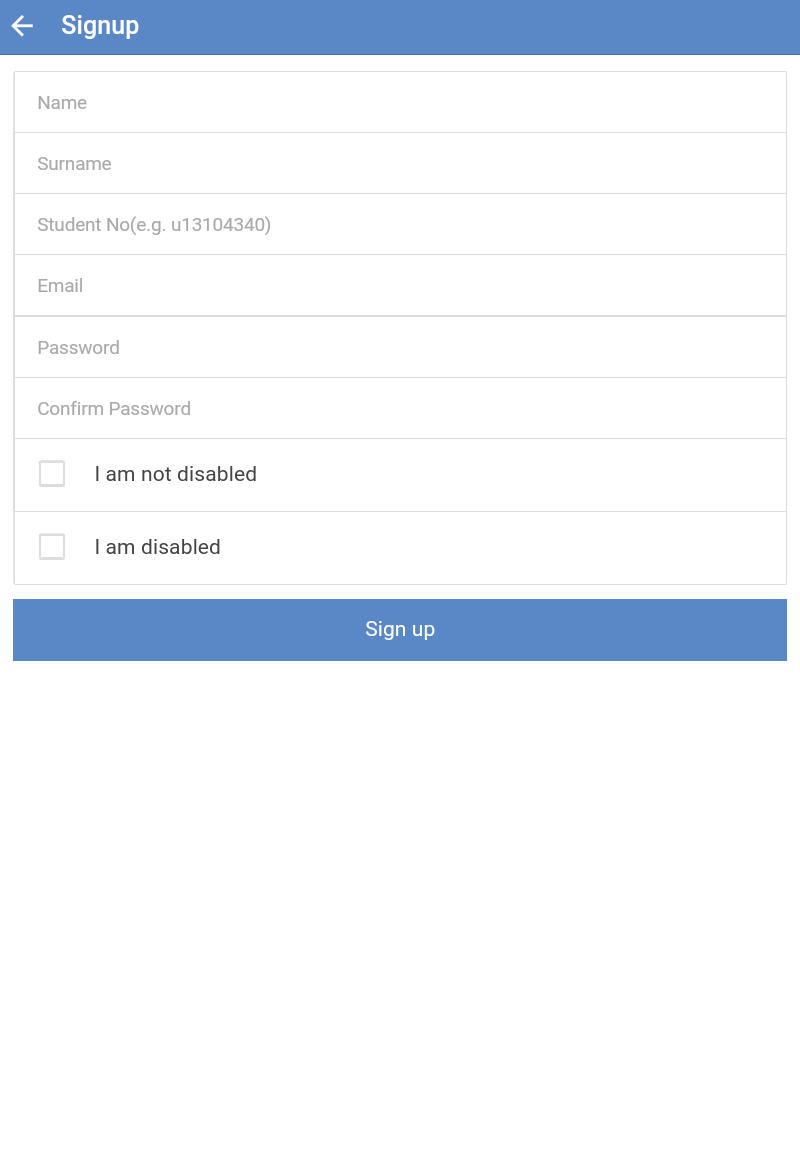
\includegraphics[height=10cm]{register.png}
	\\
	After registering successfully, users will use their student number and the password they set to gain access to the app. The login screen is shown below.
	\\
	\par
	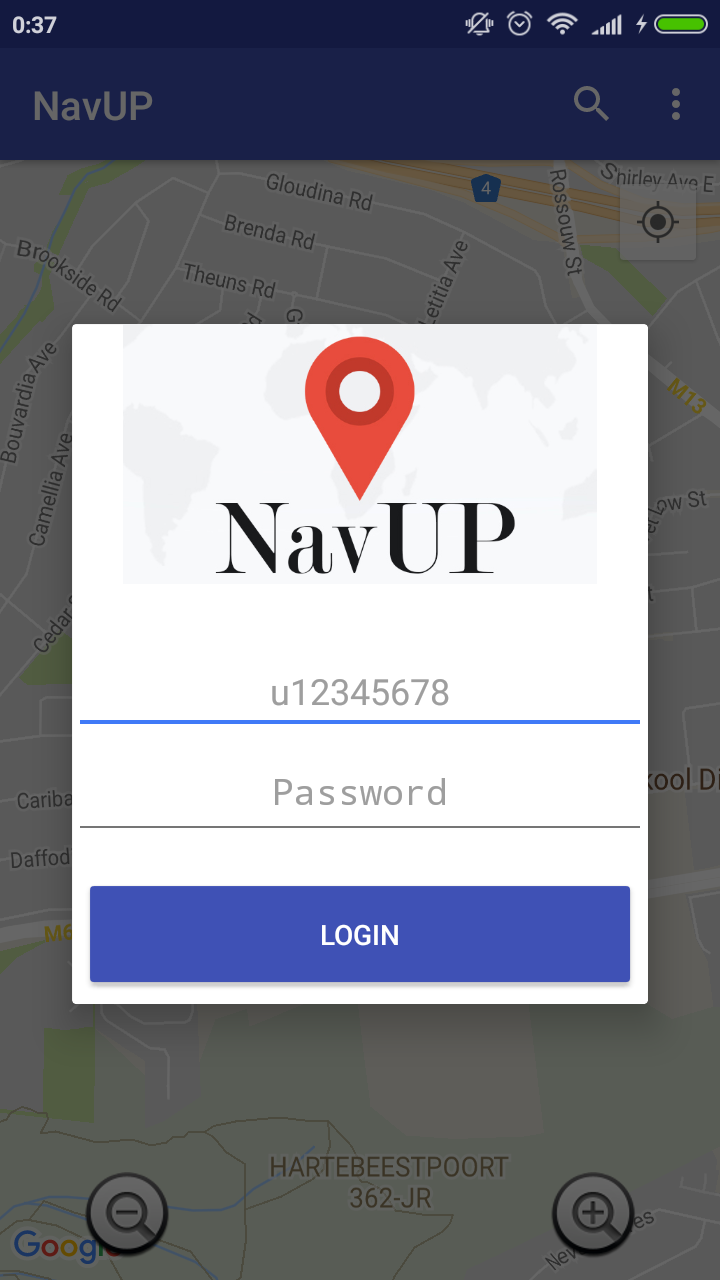
\includegraphics[height=10cm]{login.png}

\newpage
\section{Guest and User Menu}
	As previously mentioned, user can use the app as a guest with minimal functionality, the main menu for guest users is shown here below.
	\\
	\par
	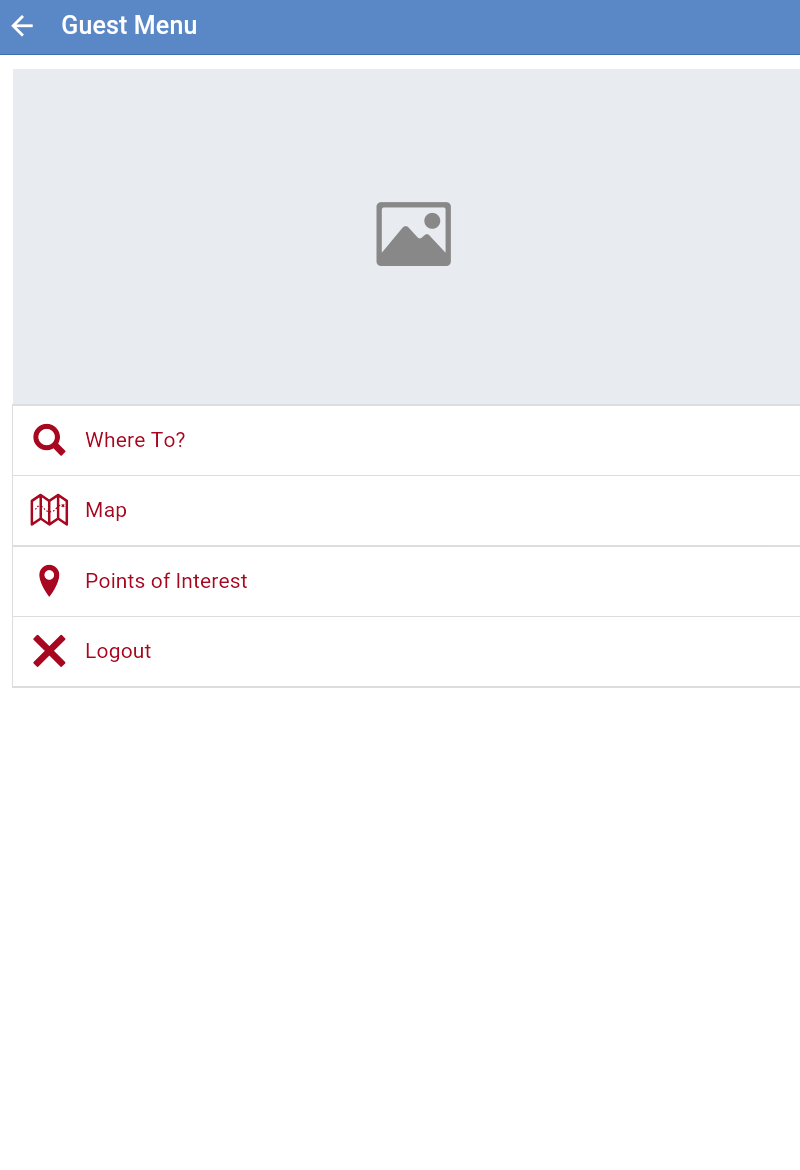
\includegraphics[height=10cm]{guestmenu.png}
	\\
	The ''Where To?'' and ''Map'' options link to pages allowing navigational functions and map views. ''Points of Interest'' is linked to a searchable list of points of interest such as food, historical buildings and so on.
	\\
	Logged in users have access to more functionality, namely a personalized and updateable timetable, a list of recently visited locations and their profile information, found under the ''Timetable'', ''Recently Visited'' and ''My Profile'' respectively. The ''Logout'' options logs the user out and terminates the session. The user menu is shown here below
	\\
	\par
	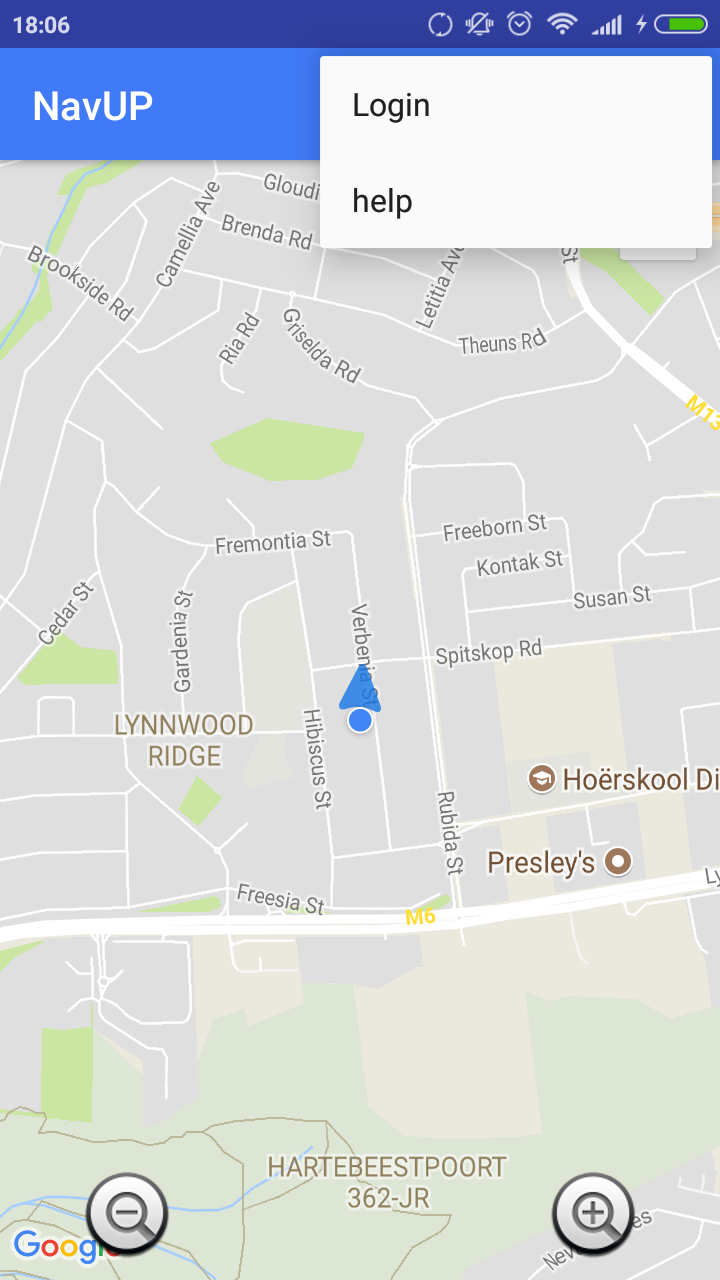
\includegraphics[height=10cm]{menu.png}
	
\newpage
\section{Navigation}
	USers wishing to navigate to a location can do so from the navigation page. This shows a map and search bar for a user's desired location. After the location is found, tap the ''Navigate'' button to determine and display the optimum route.
	\\
	\par
	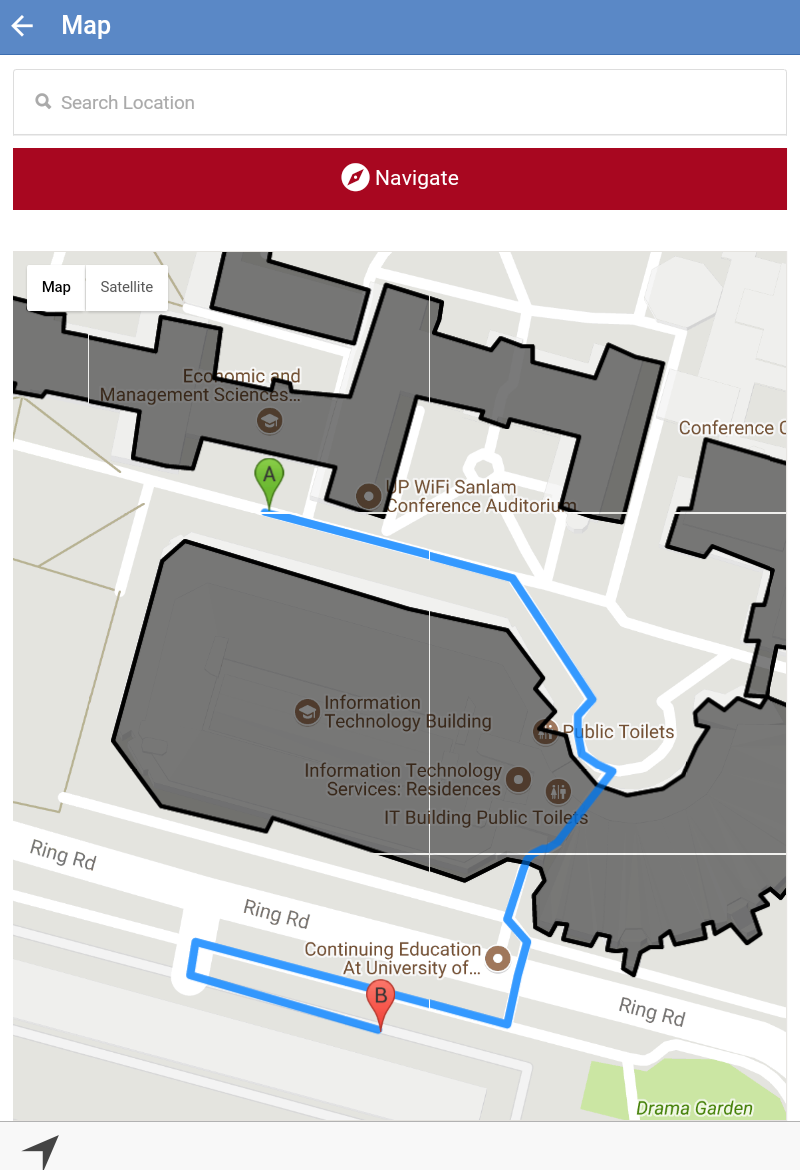
\includegraphics[height=15cm]{map.png}
\end{document}